%%%%%%%%%%%%%%%%%%%%%%%%%%%%%%%%%%%%%%%%%%%%%%%%%%%%%%%%%%%%%%%%%%%%%%%%%%%%%%%%%%%%%%%%%%%%%%%%
%
% CSCI 1430 Written Question Template
%
% This is a LaTeX document. LaTeX is a markup language for producing documents.
% Your task is to answer the questions by filling out this document, then to
% compile this into a PDF document.
%
% TO COMPILE:
% > pdflatex thisfile.tex
%
% If you do not have LaTeX and need a LaTeX distribution:
% - Departmental machines have one installed.
% - Personal laptops (all common OS): http://www.latex-project.org/get/
%
% If you need help with LaTeX, come to office hours. Or, there is plenty of help online:
% https://en.wikibooks.org/wiki/LaTeX
%
% Good luck!
% James and the 1430 staff
%
%%%%%%%%%%%%%%%%%%%%%%%%%%%%%%%%%%%%%%%%%%%%%%%%%%%%%%%%%%%%%%%%%%%%%%%%%%%%%%%%%%%%%%%%%%%%%%%%
%
% How to include two graphics on the same line:
%
% \includegraphics[width=0.49\linewidth]{yourgraphic1.png}
% \includegraphics[width=0.49\linewidth]{yourgraphic2.png}
%
% How to include equations:
%
% \begin{equation}
% y = mx+c
% \end{equation}
%
%%%%%%%%%%%%%%%%%%%%%%%%%%%%%%%%%%%%%%%%%%%%%%%%%%%%%%%%%%%%%%%%%%%%%%%%%%%%%%%%%%%%%%%%%%%%%%%%

\documentclass[11pt]{article}

\usepackage[english]{babel}
\usepackage[utf8]{inputenc}
\usepackage[colorlinks = true,
            linkcolor = blue,
            urlcolor  = blue]{hyperref}
\usepackage[a4paper,margin=1.5in]{geometry}
\usepackage{booktabs}
\usepackage{stackengine,graphicx}
\usepackage{fancyhdr}
\setlength{\headheight}{15pt}
\usepackage{microtype}
\usepackage{times}
\usepackage{amsmath}
\usepackage{amssymb}
\usepackage[shortlabels]{enumitem}
\setlist[enumerate]{topsep=0pt}

% python code format: https://github.com/olivierverdier/python-latex-highlighting
\usepackage{pythonhighlight}

\frenchspacing
\setlength{\parindent}{0cm} % Default is 15pt.
\setlength{\parskip}{0.3cm plus1mm minus1mm}

\pagestyle{fancy}
\fancyhf{}
\lhead{Project 4 Questions}
\rhead{CSCI 1430}
\lfoot{\textcolor{red}{Only
\ifcase\thepage
\or instructions and Q1
\or A1 answers
\or Q2 and A2 answers
\or Q3 and A3 answers
\or Q4 and A4 answers
\or Q5 and A5 answers
\or A5 answers
\or Q6
\or Q6
\or Q6
\or Q7 and A7 answers
\or feedback
\else
EXTRA PAGE ADDED
\fi
should be on this page
}}
\rfoot{\thepage~/ 11}

\date{}

\title{\vspace{-1cm}Project 4 Questions}


\begin{document}
\maketitle
\vspace{-2cm}
\thispagestyle{fancy}

\section*{Instructions}
\begin{itemize}
    \item 7 questions (Q6 and Q7 with code components).
    \item \emph{This will take two weeks! Parts are tricky---start early!}.
    \item Write code where appropriate; feel free to include images or equations.
    \item Please make this document anonymous.
    \item This assignment is \textbf{fixed length}, and the pages have been assigned for you in Gradescope. As a result, \textbf{please do NOT add any new pages}. We will provide ample room for you to answer the questions. If you \emph{really} wish for more space, please add a page \emph{at the end of the document}.
    \item \textbf{We do NOT expect you to fill up each page with your answer.} Some answers will only be a few sentences long, and that is okay.
    \item Question 6 has a coding component that must be submitted to Gradescope under a separate assignment (Project 4 Written Code (Numpy)) and is due a week after the rest of the written questions.
\end{itemize}

\section*{Questions}

%%%%%%%%%%%%%%%%%%%%%%%%%%%%%%%%%%%

\paragraph{Q1:} Many traditional computer vision algorithms use convolutional filters to extract feature representations, e.g., in SIFT, to which we then often apply machine learning classification techniques. Convolutional neural networks also use filters within a machine learning algorithm.

\begin{enumerate} [(a)]
    \item What is different about the construction of the filters in each of these approaches?
    \item Please declare and explain the advantages and disadvantages of these two approaches.
\end{enumerate}
\emph{Please answer on next page.}

%%%%%%%%%%%%%%%%%%%%%%%%%%%%%%%%%%%
\pagebreak
\paragraph{A1:} Your answer here.
% Uncomment the stencil below and fill in your solution.

\begin{enumerate}[(a)]

    \item In traditional computer vision algorithms, such as SIFT, the construction of filters are defined manually. For example, SIFT descriptor are constructed based upon the number in every orientation bins based upon the gradients of each pixel. However, the filters in convolutional neural networks are learned during the training process, we only need to define the shape and the number of the filters and the parameters in filters will be tuned during the optimization procedure.

    \item Filters in traditional computer vision algorithms:
          \begin{itemize}
              \item Advantages: it is fast as the feature extraction is predefined and required no training process. It is simpler design and less parameters to set compared to CNN.
              \item Disadvantages: it is poor generalization and not robust to nonlinear transformations.
          \end{itemize}
          Filters in convolutional neural network:
          \begin{itemize}
              \item Advantages: it can provide great performance in classification tasks and stongly bio-inspired and very good at generalization.
              \item Disadvantages: it requires large training set for better performance and demand high memory to store the trained weights of the network. Thus, it is slower than SIFT.
          \end{itemize}

          (source: \href{https://tams.informatik.uni-hamburg.de/lectures/2015ws/seminar/ir/pdf/slides/JosipJosifovski-Object_Recognition_SIFT_vs_Convolutional_Neural_Networks.pdf}{Object Recognition SIFT vs Convolutional Neural Networks})
\end{enumerate}


%%%%%%%%%%%%%%%%%%%%%%%%%%%%%%%%%%%
\pagebreak
\paragraph{Q2:} Many CNNs have a fully connected multi-layer perceptron (MLP) after the convolutional layers as a general purpose `decision-making' subnetwork. What effects might a \emph{locally-connected} MLP have on computer vision applications, and why?

Please give your answer in terms of the learned convolution feature maps, their connections, and the perceptrons in the MLP.

%%%%%%%%%%%%%%%%%%%%%%%%%%%%%%%%%%%
\paragraph{A2:}

In convolutional neural network, for each position (x, y), the dot product summation between the kernel and image values around the point is calculated for next layer. For the whole image, the kernel will remain the same everywhere, which means the weights is shared among the whole image. However, for \emph{locally-connected} MLP, for each position (x,y), it will have its private kernel filter whose weights is not shared globally.

Comparing these two methods, for CNN, we tend to miss out on some subtle nuances of spatial arrangements as the features are learned using the filter that applies to the whole image. Using \emph{locally-connected} MLP might be helpful for such subtle differences detections. For the connections, the connections are similar but for CNN we are having filtering moving across the image while for \emph{locally-connected} MLP, we have different filters at each position. In terms of the preceptrons in the MLP, with weights unshared and being private to each pixel, \emph{locally-connected} MLP will need more filters to be trained compared to the CNN model.

Source: \href{https://prateekvjoshi.com/2016/04/12/understanding-locally-connected-layers-in-convolutional-neural-networks/}{Understanding Locally Connected Layers In Convolutional Neural Networks}
%%%%%%%%%%%%%%%%%%%%%%%%%%%%%%%%%%%

\pagebreak
\paragraph{Q3:} Given a neural network and the stochastic gradient descent training approach for that classifier, discuss how the \emph{learning rate}, \emph{batch size}, and \emph{training time} hyperparameters might affect the training process and outcome.

%%%%%%%%%%%%%%%%%%%%%%%%%%%%%%%%%%%
\paragraph{A3:} Your answer here.
% Uncomment the stencil below and fill in your solution.

\begin{enumerate}[(a)]

    \item \emph{learning rate}: the learning rate controls how fast the model is adpated to the problem. Smaller learning rate requires more training epochs as the smaller changes are made to tune the weights of the model, whereas larger learning rates result in rapid change and require fewer epochs. For the outcome, if the learning rate is too large it can cause the model converge too quickly to a suboptimal solution or diverged, whereas a too small learning rate might cause the process to get stuck.

    \item \emph{batch size}: the batch size impacts how quickly a model learns and the stability of the learning process. A smaller batch size are noisy, offering a regularizaing effect and lower generalization error while require less memory for training model. A larger batch size will lead to poor generalization but using a batch equal to the entire dataset guarantees convergence to the global optima of the objective function.

          (Source: \href{https://machinelearningmastery.com/how-to-control-the-speed-and-stability-of-training-neural-networks-with-gradient-descent-batch-size/}{How to control the stability of training neural networks with the batch size}; \href{https://medium.com/mini-distill/effect-of-batch-size-on-training-dynamics-21c14f7a716e}{Effect of batch size on training dynamics})
    \item \emph{training time}: generally the training epochs will decide the training time of the model. If the number of training epochs is too small, the model might not reach the optima and give a bad performance. If the number of training epochs is too large, the model might become overfitting to the training data and start to lose performance in terms of generalization to test data.

\end{enumerate}


%%%%%%%%%%%%%%%%%%%%%%%%%%%%%%%%%%%%%%%%%%%%%%%%%%%%
\pagebreak
\paragraph{Q4:} What effects does adding a max pooling layer have for a single convolutional layer, where the output with max pooling is some size larger than 1 x 1 x d?

\emph{Notes:} 'Global' here means whole image; 'local' means only in some image region.

\emph{LaTeX:} To fill in boxes, replace `\textbackslash square' with `\textbackslash blacksquare' for your answer.

\paragraph{A4:} Multiple choice. Choose all that apply.

%%% See the tex for the bottom of the page to leave the optional written justification %%%
\begin{tabular}[h]{lr}
    \toprule
    Increases computational cost of training            & $\square$      \\
    Decreases computational cost of training            & $\blacksquare$ \\
    Increases computational cost of testing             & $\square$      \\
    Decreases computational cost of testing             & $\blacksquare$ \\
    \midrule
    Increases overfitting                               & $\square$      \\
    Decreases overfitting                               & $\blacksquare$ \\
    Increases underfitting                              & $\blacksquare$ \\
    Decreases underfitting                              & $\square$      \\
    \midrule
    Increases the nonlinearity of the decision function & $\square$      \\
    Decreases the nonlinearity of the decision function & $\blacksquare$ \\
    \midrule
    Provides local rotational invariance                & $\blacksquare$ \\
    Provides global rotational invariance               & $\square$      \\
    Provides local scale invariance                     & $\square$      \\
    Provides global scale invariance                    & $\square$      \\
    Provides local translational invariance             & $\blacksquare$ \\
    Provides global translational invariance            & $\square$      \\
    \bottomrule
\end{tabular}


%%%%%%%%%%%%%%%%%%%%%%%%%%%%%%%%%%%%%
\paragraph{Something to think about (ungraded):} Given some input to a convolutional layer with stride 2$\times$2 and kernel size 3$\times$3, and ignoring the boundary, what is the minimum number of convolutional filters required to preserve all input information in the output feature map?

%%%%%%%%%%%%%%%%%%%%%%%%%%%%%%%%%%%
Multiple choice.
\emph{LaTeX:} Use command  `\textbackslash bullet' ($\bullet$) to fill in the dots.

\begin{tabular}[h]{lc}
    \toprule
    0.5             & $\square$ \\
    1               & $\bullet$ \\
    2               & $\square$ \\
    4               & $\square$ \\
    It's impossible & $\square$ \\
    \bottomrule
\end{tabular}
%%%%%%%%%%%%%%%%%%%%%%%%%%%%%%%%%%%%%

% Space for optional justification. Do NOT go past this page!
\emph{Here:} Feel free to leave optional short written justification if desired.

%%%%%%%%%%%%%%%%%%%%%%%%%%%%%%%%%%%
\pagebreak
\paragraph{Q5:}
In medical imaging, hand designing features with biological experts might lead to a generalizable and explainable method for physicians, regulators, or patients. However, deep learning methods can show higher test accuracy, even if their results may be less explainable.
Please read this \href{https://drive.google.com/file/d/16CztlicOOTImvP9ZrtTUNKwLuv6srOBW/view?usp=sharing}{short article}.

\begin{enumerate}[(a)]
    \item
          In the article, physician Dr. Nicholas Price expresses the view that a lack of explainability should not hamper advances in health care, pointing out that Aspirin’s mechanism was not understood for 70 years and that Lithium’s mechanism to treat bipolar disorder is still unknown. Do you agree with Dr. Price? Would you feel comfortable allowing your doctor to rely on a ‘black box’ algorithm for medical diagnoses? (3-4 sentences)
    \item
          When deciding whether a medical algorithm is suitable for clinical use, what accuracy would you consider to be ‘good enough’? In which different ways could we measure this? (3-4 sentences)
    \item
          In the event that a medical imaging algorithm makes an error and causes a patient harm, who should be held responsible? \textit{Think about everyone involved: the algorithm engineer, the company selling the algorithm, the FDA approving it, the hospital or clinic purchasing it, the physician using it, etc.} (3-4 sentences)
    \item
          Nicholas Price is actually a \href{https://drive.google.com/file/d/1bDAqEtW482OJeqMBt5A4AradVa4gf_o9/view}{legal scholar} who specializes in health law at the University of Michigan. Does this information change your responses? (3-4 sentences)

\end{enumerate}

%%%%%%%%%%%%%%%%%%%%%%%%%%%%%%%%%%%
\paragraph{A5:} Your answer here.
% Uncomment the stencil below and fill in your solution.

\begin{enumerate}[(a)]

    \item No, I don't agree with Dr. Price. Although the mechanisms of Aspirin and Lithium are not understood yet, they both show consistent positive results to patients, or at least no negative effects to the patients. However, for DL algorithms there still exists possibilities for the false predictions. And once it gives a false prediction, it will lead to some irreparable results.

          I don't feel comfortable using a ‘black box’ algorithm for my medical diagnoses. I would not know the reason why it gives such diagnoses and I don't feel that I could trust it.

    \item To be ‘good enough’, the accuracy of the algorithm should reach at least 99.99\%. That is 1 false prediction out of 10000 results. These is still really large if we take the number of patients into consideration. There are 7 billion people around the world and if they all use this algorithm to diagonize the disease, there will be 70,000 false predictions.

          We could measure the percentage of false negatives as this is actually the worst case for the patients when the model gives predictions. And it would be easier to lower this percentage than the whole accuracy.

          %%%%%%%%%%%%%%%%%%%%%%%%%%%%%%%%%%%

          \pagebreak
          Extra page. Please remember to keep your page length the same.

    \item First of all, the physicians using the medical imaging algorithm will remain ultimately responsible for patient care. They need to acquire new skills to do their best for patients before they decide whether or not to adopt the outcome of the algorithms. Second, the company selling the algorithm and the hospital or clinic purchasing it share the same responsibilities as they are the ones that write the code and introduce them to physicians. Lastly, the FDA has to reexamine the safety of this algorithm and redesign their procedure for such AI algorithms approving.

    \item This information doesn't change my responses. Although Dr. Nicholas is knowledgable of the field of public health, his opionion can be affected by his personal emotions. There are so many cases where experts hold contradictory views to the same things and some of them should be wrong. Before the wide application of deep learning in health field, I would prefer it has gone through careful and meticulous testing.
\end{enumerate}

% Please leave the pagebreak
\pagebreak
%%%%%%%%%%%%%%%%%%%%%%%%%%%%%%%%%%%%%
\paragraph{Q6 background:}
Let us consider using a neural network (non-convolutional) to perform classification on the \href{http://yann.lecun.com/exdb/mnist/}{MNIST dataset} of handwritten digits, with 10 classes covering the digits 0--9. Each image is 28$\times$28 pixels, and so the network input is a 784-dimensional vector $\mathbf{x}=(x_1,x_2,\dots,x_i,\dots,x_{784})$. The output of the neural network is probability distribution $\mathbf{p}=(p_1,\dots,p_j,\dots,p_{10})$ over the 10 classes. Suppose our network has one fully-connected layer with $10$ neurons---one for each class. Each neuron has a weight for each input $\mathbf{w}=(w_1,\dots,w_i,\dots,w_{784})$, plus a bias $b$. As we only have one layer with no multi-layer composition, there's no need to use an activation function.

When we pass in a vector $\mathbf{x}$ to this layer, we will compute a 10-dimensional output vector $\mathbf{l}=(l_1,l_2,...,l_j,...,l_{10})$ as:
\begin{equation}
    l_j = \mathbf{w}_j \cdot \mathbf{x} + b_j = \sum_{i=1}^{784}w_{ij}x_i + b_j
\end{equation}
These distances from the hyperplane are sometimes called `logits' (hence $l$) when they are the output of the last layer of a network. In our case, we only have \emph{one} layer, so our single layer is the last layer.

\hspace{\fill}\rule{0.5\linewidth}{.5pt}\hspace{\fill}

Often we want to talk about the confidence of a classification. So, to turn our logits into a probability distribution $\mathbf{p}$ for our ten classes, we apply the \emph{softmax} function:
\begin{equation}
    p_j = \frac{e^{l_j}}{\sum_je^{l_j}}
    \label{eq:softmax}
\end{equation}
Each $p_j$ will be positive, and $\sum_jp_j = 1$, and so softmax is guaranteed to output a probability distribution. Picking the most probable class provides our network's prediction.

\emph{If} our weights and biases were trained, Eq.~\ref{eq:softmax} would classify a new test example.

\hspace{\fill}\rule{0.5\linewidth}{.5pt}\hspace{\fill}

We have two probability distributions: the true distribution of answers from our training labels $\mathbf{y}$, and the predicted distribution produced by our current classifier $\mathbf{p}$. To train our network, our goal is to define a loss to reduce the distance between these distributions.

Let $y_j=1$ if class $j$ is the true label for $x$, and $y_j = 0$ if $j$ is not the true label. Then, we define the \emph{cross-entropy loss}:
\begin{equation}
    L(w,b,x) = - \sum_{j=1}^{10}y_j\ln(p_j),
\end{equation}
which, after substitution of Eqs. 2 and 1, lets us compute an error between the labeled ground truth distribution and our predicted distribution.

So...why does this loss $L$ work? Using the cross-entropy loss exploits concepts from information theory---Aur\'{e}lien G\'{e}ron has produced \href{https://www.youtube.com/watch?v=ErfnhcEV1O8}{a video with a succinct explanation of this loss}. Briefly, the loss minimizes the difference in the amounts of information needed to represent the two distributions. Other losses are also applicable, with their own interpretations, but these details are beyond the scope of this course.

%%%%%%%%%%%%%%%%%%%
% Cheat sheet for information theory
%
% Probability distribution \mathbf{p}
% Describes the likelihood of different outcomes, e.g., for our MNIST dataset samples, we might have a 0.09 chance that an image will be of a character '0', 0.11 for a '1', 0.08 for a '2', and so on, with the sum chances for all characters being 1.0.
%
% What is entropy?  H(\mathbf{p}) = - \sum_{i} p_i \log_2{p_i}
% Probability of an event multiplied by the reduction in uncertainty (or amount of information) received from that event. Is the average amount of information (in bits) that you receive from one sample drawn from a probability distribution. It tells you how predictable that probability distribution is (or, written another way, how uncertain we are). 0 entropy = no uncertainty. High entropy = very uncertain probability distribution.
%
% What is cross-entropy?   H(\mathbf{p},\mathbf{q}) = - \sum_{i} p_i \log_2{q_i}
% The average message length in bits _across_ two distributions - the true distribution \mathbf{p} and some predicted distribution \mathbf{q}. If the predicted distribution is equal to the true distribution, then cross-entropy _is_ entropy.
%
% So then what is entropy minus cross-entropy?
% This tells us how different the predicted distribution is from the true distribution. This is called the Kullback-Leibler divergence (or KL-divergence). It is a divergence and not a distance because it doesn't have a 'sidedness'.
% D_{KL}(\mathbf{p} || \mathbf{q}) = H(\mathbf{p},\mathbf{q}) - H(\mathbf{p})
%
% Why is it \emph{minus}?   The uncertainty reduction factor from a message is equal to 1 / p(event). So, we would normally compute ln( 1/p(event) ). But ln(1/x) = -ln(x), so we equivalently compute -ln( p(event) ).
%
%%%%%%%%%%%%%%%%%%%

\hspace{\fill}\rule{0.5\linewidth}{.5pt}\hspace{\fill}

Onto the training algorithm. The loss is computed once for every different training example. When every training example has been presented to the training process, we call this an \emph{epoch}. Typically we will train for many epochs until our loss over all training examples is minimized.

Neural networks are usually optimized using gradient descent. For each training example in each epoch, we compute gradients via backpropagation (an application of the chain rule in differentiation) to update the classifier parameters via a learning rate $\lambda$:
\begin{equation}
    w_{ij} = w_{ij} - \lambda\frac{\partial L}{\partial w_{ij}}, \\
\end{equation}
\begin{equation}
    b_j = b_j - \lambda\frac{\partial L}{\partial b_j}.
\end{equation}

We must deduce $\frac{\partial L}{\partial w_{ij}}$ and $\frac{\partial L}{\partial b_j}$ as expressions in terms of $x_i$ and $p_j$.

\emph{Intuition:} Let's just consider the weights. Recall that our network has one layer of neurons followed by a softmax function. To compute the change in the cross-entropy loss with respect to neuron weights $\frac{\partial L}{\partial w_{ij}}$, we will need to compute and chain together three different terms:
\begin{enumerate}
    \itemsep0em
          \listparindent0em
          \topsep0em
          \parsep0em
          \partopsep0em
    \item the change in the loss with respect to the softmax output $\frac{\delta L}{\delta p_j}$,
    \item the change in the softmax output with respect to the neuron output $\frac{\delta p_j}{\delta l_j}$, and
    \item the change in the neuron output with respect to the neuron weights $\frac{\delta l_j}{w_{ij}}$.
\end{enumerate}
We must derive each individually, and then formulate the final term via the chain rule. The biases follow in a similar fashion.

The derivation is beyond the scope of this class, and so we provide them here:
\begin{equation}
    \frac{\delta L}{\delta w_{ij}} = \frac{\delta L}{\delta p_a} \frac{\delta p_a}{\delta l_j} \frac{\delta l_j}{w_{ij}} =\begin{cases}
        x_i(p_j-1), a = j \\
        x_ip_j,  a\neq j
    \end{cases}
    \label{eq:wupdate}
\end{equation}
\begin{equation}
    \frac{\delta L}{\delta b_j} = \frac{\delta L}{\delta p_a} \frac{\delta p_a}{\delta l_j} \frac{\delta l_j}{b_j} =\begin{cases}
        (p_j-1), a = j \\
        p_j,  a\neq j
    \end{cases}
    \label{eq:bupdate}
\end{equation}
Here, $a$ is the predicted class label and $j$ is the true class label. An alternative form you might see shows $\frac{\delta L}{\delta w_{ij}} = x_i(p_j-y_j)$ and $\frac{\delta L}{\delta b_j} = p_j-y_j$ where $y_j=1$ if class $j$ is the true label for $x$, and $y_j = 0$ if $j$ is not the true label.

So...after all of that, our gradient update rules are surprisingly simple!

\emph{Further details:} For interested students, we refer students to Chapter 1 of \href{https://cs.brown.edu/courses/csci1460/assets/files/deep-learning.pdf}{Prof.~Charniak's deep learning notes}, which derives these gradient update rules. We also refer to \href{https://www.ics.uci.edu/~pjsadows/notes.pdf}{Prof.~Sadowski's notes on backpropagation}: Section 1 derives terms first for cross-entropy loss with logistic (sigmoid) activation, and then Section 2 derives terms for cross-entropy loss with softmax. The Wikipedia article on \href{https://en.wikipedia.org/wiki/Backpropagation}{the backpropagation algorithm} likewise represents a derivation walkthrough of the general case with many hidden layers each with sigmoid activation functions, and a final layer with a softmax function.

\hspace{\fill}\rule{0.5\linewidth}{.5pt}\hspace{\fill}


\paragraph{Q6:} We will implement these steps in code using numpy. We provide a code stencil \texttt{main.py} which loads one of two datasets: MINST and the scene recognition dataset from Project 3. We also provide two models: a neural network, and then a neural network whose logits are used as input to an SVM classifier. Please look at the comments in \texttt{main.py} for the arguments to pass in to the program for each condition. The neural network model is defined in \texttt{model.py}, and the parts we must implement are marked with TODO comments.

\emph{Tasks:} Please follow the steps to implement the forward model evaluation and backward gradient update steps. Then, run your model on all four conditions and report training loss and accuracy as the number of training epochs increases.


Please upload your completed \texttt{model.py} to Gradescope under the assignment titled "Project 4 Written Code (Numpy)". The autograder will check that you correctly implemented parts of your model. Please also include a \texttt{writeup.pdf} with your responses to the following questions.

\begin{enumerate}
    \item What do these numbers tell us about the capacity of the network, the complexity of the two problems, the value of training, and the value of the two different classification approaches?

    \item How well did each model perform on each dataset? Please use this table to structure your response.

          \begin{itemize}
              \item NN on MNIST: xx\% (highest accuracy)
                    \begin{itemize}
                        \item Epoch 0 loss: xx     Accuracy: xx\%
                        \item Epoch 9 loss: xx     Accuracy: xx\%
                    \end{itemize}
              \item NN+SVM on MNIST: xx\% (highest accuracy)
                    \begin{itemize}
                        \item Epoch 0 loss: xx     Accuracy: xx\%
                        \item Epoch 9 loss: xx     Accuracy: xx\%
                    \end{itemize}
              \item NN on SceneRec: xx\% (highest accuracy)
                    \begin{itemize}
                        \item Epoch 0 loss: xx     Accuracy: xx\%
                        \item Epoch 9 loss: xx     Accuracy: xx\%
                    \end{itemize}
              \item NN+SVM on SceneRec: xx\% (highest accuracy)
                    \begin{itemize}
                        \item Epoch 0 loss: xx     Accuracy: xx\%
                        \item Epoch 9 loss: xx     Accuracy: xx\%
                              s\end{itemize}
          \end{itemize}

\end{enumerate}

%%%%%%%%%%%%%%%%%%%%%%%%%%%%%%%%%%%

\pagebreak
\paragraph{Q7:} Follow the \href{https://browncsci1430.github.io/webpage/resources/gcp_guide/}{GCP guide} to set up GCP. \emph{Note:} This is tricky, and it will take you some time to become familiar with the system! Once finished, complete one of these two Tensorflow MNIST tutorials on GCP:
\begin{itemize}
    \item \href{https://www.tensorflow.org/tutorials/quickstart/beginner}{TensorFlow 2 quickstart for beginners}
    \item \href{https://www.tensorflow.org/tutorials/quickstart/advanced}{TensorFlow 2 quickstart for experts}
\end{itemize}

The work for the tutorial can be done in a completely new Python file inside or outside of your project code (you won't have to turn it in).


%%%%%%%%%%%%%%%%%%%%%%%%%%%%%%%%%%%
\paragraph{A7:} Please insert a screenshot of the tutorial code output, running on GCP:

I choose to finish the second one \href{https://www.tensorflow.org/tutorials/quickstart/advanced}{TensorFlow 2 quickstart for experts}. From the screenshot, we can check that GPU is K80 and accuracy results meets our expectation.
\begin{figure}[htbp]
    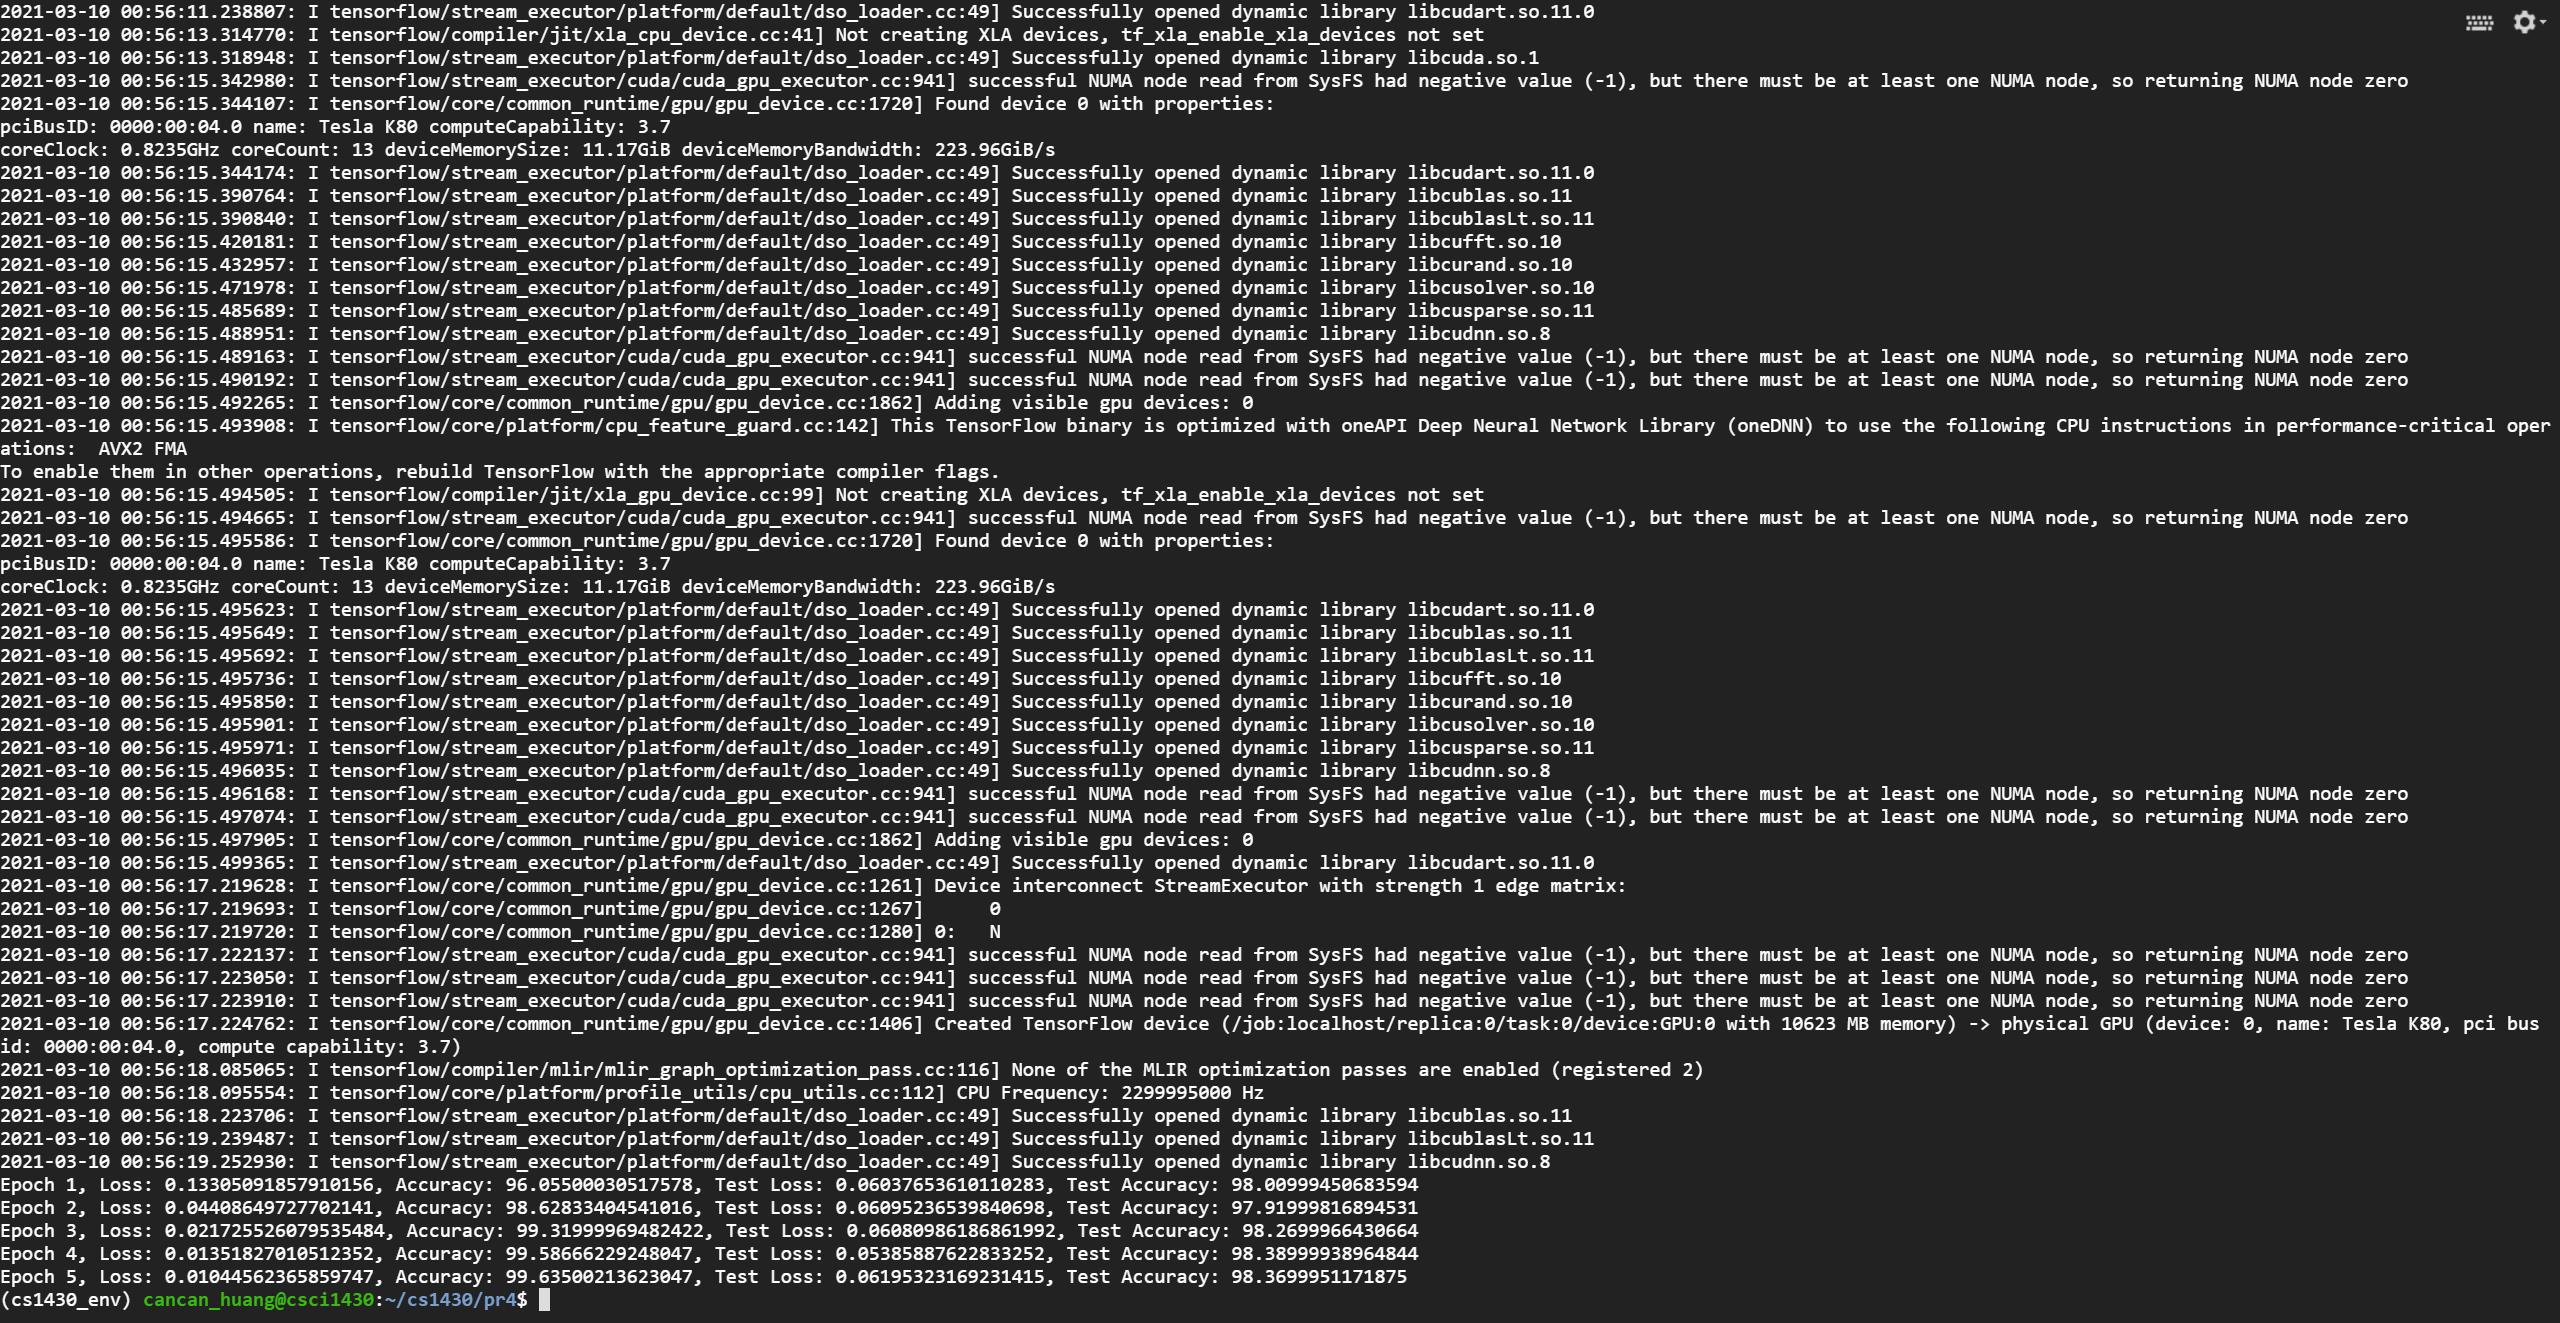
\includegraphics[width=\linewidth]{Q7.png}
\end{figure}


%%%%%%%%%%%%%%%%%%%%%%%%%%%%%%%%%%%


%%%%%%%%%%%%%%%%%%%%%%%%%%%%%%%%%%%
\pagebreak
\section*{Feedback? (Optional)}
Please help us make the course better. If you have any feedback for this assignment, we'd love to hear it!


% \pagebreak
% \section*{Any additional pages would go here.}


\end{document}
